% This is samplepaper.tex, a sample chapter demonstrating the
% LLNCS macro package for Springer Computer Science proceedings;
% Version 2.21 of 2022/01/12
%
\documentclass[runningheads]{llncs}
%
\usepackage[T1]{fontenc}
% T1 fonts will be used to generate the final print and online PDFs,
% so please use T1 fonts in your manuscript whenever possible.
% Other font encondings may result in incorrect characters.
%
\usepackage{graphicx}
\usepackage[table,xcdraw]{xcolor}
\usepackage{helvet,times,courier}
\usepackage{multirow}
\usepackage{algorithm2e}
\SetKwInput{KwParam}{Parameters}
\SetKw{KwFrom}{from}
\SetCommentSty{textit}

\usepackage{graphicx}
% Used for displaying a sample figure. If possible, figure files should
% be included in EPS format.
%
% If you use the hyperref package, please uncomment the following two lines
% to display URLs in blue roman font according to Springer's eBook style:
%\usepackage{color}
%\renewcommand\UrlFont{\color{blue}\rmfamily}
%\urlstyle{rm}
%
\sloppy
\hyphenation{make-span}
\begin{document}
%
\title{Swarm Intelligence-Driven Dispatching Rules for Large-Scale Semiconductor Production: Integrating Simulation and Optimization to Enhance Operational Efficiency
}
%
%\titlerunning{Abbreviated paper title}
% If the paper title is too long for the running head, you can set
% an abbreviated paper title here
%
\author{Ramsha Ali\inst{1}\orcidID{0000-0002-4794-6560} \and
Peyman Eftekhari\inst{1}\orcidID{0009-0007-4198-392X} \and
Martin Gebser\inst{1}\orcidID{0000-0002-8010-4752} \and
Stephan Leitner\inst{2}\orcidID{0000-0001-6790-4651} \and
Gerhard Friedrich\inst{1}\orcidID{0000-0002-1992-4049}
}
%
\authorrunning{R. Author et al.}
% First names are abbreviated in the running head.
% If there are more than two authors, 'et al.' is used.
%
\institute{Department of Artificial Intelligence and Cybersecurity, \and
	Department of Management Control and Strategic Management, \\ University of Klagenfurt, Austria \\
	\email{\{ramsha.ali,peyman.eftekhari,martin.gebser, \\ stephan.leitner,gerhard.friedrich\}@aau.at} \\
	\url{https://www.aau.at}}

%
\maketitle              % typeset the header of the contribution
%
\begin{abstract}
The abstract should briefly summarize the contents of the paper in
150--250 words.

\keywords{Swarm intelligence \and Ant colony optimization \and Greedy search \and Semiconductor production \and Scheduling \and Dispatching \and Simulation}
\end{abstract}
%
%
%
\section{Introduction}
\label{sec:introduction}
As the digital transformation deepens across various sectors, the demand for more powerful, energy-efficient, and smaller semiconductors continues to escalate. This surge in demand places immense pressure on semiconductor manufacturers to scale up production without compromising quality. Semiconductor production involves hundreds of sophisticated steps, each of which must be precisely controlled to ensure the functionality and yield of the final product \cite{kopp2020smt2020}. The complexity is exacerbated by the rapid pace of innovation in semiconductor design, which frequently shifts production parameters and process requirements.

Dispatching in semiconductor production is a particularly challenging aspect of factory operations. It involves determining the sequence and timing of various production tasks, from wafer fabrication to assembly and testing, to maximize throughput \cite{Hopp2011}. In large-scale operations, the complexity is magnified by the sheer number of variables involved, including machine availability, maintenance schedules, workforce shifts, and rapidly changing order priorities. Traditional dispatching solutions often fall short in such an environment, as they cannot adequately adapt to the dynamic and complex nature of semiconductor production. This inadequacy can lead to sub-optimal decisions that compromise operational efficiency and product quality \cite{Uzsoy1992}.

On the other hand, scheduling in large-scale semiconductor production is a cornerstone of operational management that directly influences the effectiveness and efficiency of the entire manufacturing process \cite{schumann2022scheduling}. It involves planning and organizing production activities to ensure that resources are utilized optimally and product flows are synchronized across various stages of the manufacturing process. Effective scheduling is critical not only for maintaining high throughput but also for minimizing production delays and reducing inventory and holding costs.

The scheduling of semiconductor manufacturing is notably complex due to the high variability in production processes, the sensitive nature of the materials involved, and the stringent quality requirements \cite{May2006}. Each semiconductor product may pass through hundreds of processing steps, requiring precise timing and coordination. Moreover, the high mix of product types, each with different processing needs and priorities, adds another layer of complexity \cite{Mönch2011}. This complexity is further exacerbated by the need to integrate new product introductions seamlessly into the production schedule without disrupting ongoing operations.

Scheduling production operations within the intricate landscape of semiconductor manufacturing represents one of the most daunting challenges in resource allocation. The dynamic nature of manufacturing environments—characterized by unpredictable fluctuations in process and demand, supply chain delays, and frequent machine breakdowns—significantly intensifies this complexity. Consequently, production scheduling must not only strive for near-optimal outcomes but also maintain robustness and flexibility to adapt swiftly to frequent changes in the production landscape.     

In this paper, we address a large-scale Semiconductor Manufacturing Scheduling Problem (SMSP) \cite{kopp2020smt2020}, called fab for short, is a complex production environment characterized by customized job flows and high-tech machines.

Modern semiconductor fabs process tens of thousands of operations per day using more than 1000 machines \cite{kopp2020smt2020}.
These machines are organized in tool groups with specific functionalities,
e.g., diffusion, etching, or metrology,
and each manufacturing step can be flexibly allocated to a machine 
providing the required functionality.
Hence, the scheduling of semiconductor production operations consists of the
sub-tasks of assigning operations to machines and sequencing the operations on each machine.
However, in case of machine breakdowns or process deviations,
a schedule must be revised to adapt to the changed environment.

To this end, we proposed a Greedy Search based Ant Colony Optimization (GSACO)
algorithm for (re-)scheduling semiconductor production operations \cite{Ali2024}. 
Our algorithm harnesses Ant Colony Optimization (ACO) \cite{Dorigo2019} for exploration, while
Greedy Search (GS) \cite{Papadimitriou} enables responses in short time. 
% In fact, we show that
In this way,
GSACO overcomes limitations of a
state-of-the-art Constraint Programming approach \cite{Perron2023}
on large-scale SMSP % semiconductor manufacturing scheduling 
instances. 

In our previous research \cite{Ali2024}, we introduced a novel approach that synergistically combines probabilistic operation sequencing with a greedy machine assignment strategy, targeting up to five operations per lot with the primary objective of minimizing makespan. Building on this foundational work, the current paper extends these initial concepts by proposing an enhanced algorithm, GSACO-1, specifically designed to optimize operational throughput. This development marks a significant advancement in our methodology, aiming to refine the dispatching rules further though simulation.

The paper is organized as follows. 
Section~\ref{sec:lit_rev} provides literature reviews on FJSSP and ACO.
In Section~\ref{sec:problem_f}, we formulate SMSP in terms of the well-known FJSSP. 
% and Section \ref{sec:aco} describes the overview of the ACO approach. 
Our GSACO-1 algorithm is presented in Section~\ref{sec:gsaco}.
In Section~\ref{sec:sim} we present the customized simulation adopted from \cite{Kovács2022}.
Section~\ref{sec:results} provides and discusses experimental results.
Finally, Section~\ref{sec:conclusion} concludes the paper.

\section{literature Review}
\label{sec:lit_rev}
We briefly survey the relevant literature on the challenges inherent in SMSP, a sector marked by its complex operational dynamics and the critical need for highly efficient dispatching systems. Semiconductor production processes are characterized by their high variability, sophisticated product mixes, and stringent quality demands, which collectively necessitate innovative approaches to production scheduling and dispatching. 
Later, we survey the relevant literature on methods for FJSSP, which we use as general
scheduling model to represent semiconductor production processes and SMSP.
Then we explore the traditional dispatching methods detailing their advantages and limitations within the context of semiconductor fabrication facilities. These conventional methods form the baseline against which the efficacy of advanced dispatching techniques, particularly those driven by Swarm Intelligence (SI), are evaluated. Furthermore, the review will cover essential performance metrics traditionally used to assess the effectiveness of dispatching rules.
%This section represents a brief relevant literature on the Flexible Job Shop Scheduling Problem (FJSSP), which was initially used as a general scheduling model for semiconductor production. Alternatively, this moves on with a discussion around the Semiconductor Manufacturing Scheduling Problem (SMSP), and how it can proceed with Ant Colony Optimization (ACO) and the solution.
\subsection{Semiconductor Manufacturing Scheduling Problem (SMSP)}
Semiconductor manufacturing is characterized by its complex multi-step fabrication process, each involving highly precise and controlled conditions. The fabrication of semiconductor devices often requires hundreds of steps during the photolithography, etching, and chemical deposition phases, among others. This complexity is compounded by the requirement for extremely clean environments to avoid contamination of the microscopically small circuits, making operational excellence a challenging goal \cite{May2006}.

Unlike other manufacturing industries that produce a limited range of products, semiconductor manufacturers typically deal with a high mix of products on the same production line. This high mix coupled with the rapid product evolution typical of the tech industry results in significant fluctuations in production volumes. Manufacturers must, therefore, be highly responsive to changes in demand and technology without compromising on the speed or quality of production .

The SMSP is a complex and critical challenge to optimize scheduling tasks during the manufacturing process of a semiconductor. Different methods have been adopted for a long time for varied types of machines \cite{chan2024situation}. The core aspects include job scheduling, batch processing, priority constraints, setup times of the machine, machine availability, and reentrant flow. The key challenges stay with complexity, dynamic job arrivals, and reducing downtime while maximizing throughput \cite{el2023}. Many researchers and developers have been working on the topic and suggested their methods to solve the problem.

%Mixed-integer linear programming (MILP) is a great option to solve large mathematical problems by optimizing the solution. As suggested by \cite{fang2023problems} in their study to identify important research problems with semiconductor manufacturing operations (SMOs), MILP models are extensively used in deterministic SMO scheduling problems. While MILP models are great for optimal solutions for small-scale instances, these models can also be used to provide upper bounds for large-scale instances. The only thing is, there is no optimal solution for such situations, but it is done by relaxing several constraints. 

%Another paper \cite{wang2014hybrid} was written for research of an SMSP to solve all the constraints of the semiconductor manufacturing industry such as machine status, setup time, limited waiting time, different process times on varied machines, and more. The researchers suggested a hybrid estimation of a distribution algorithm with multiple subpopulations (HEDA-MS) to solve SMSP and to make the total exceed the limited waiting time to zero.


\subsection{Flexible Job Shop Scheduling}
Considering the manufacturing industry, FJSSP is a common problem, especially for small batch and custom productions. The mathematical models allow us to solve the optimality issue for small-scale instances. As \cite{dauzere2024flexible} explains, it is important to assign the FJSSP on a machine in a particular sequence. As the optimization criteria need the start time of all the operations, it is important to optimize the completion time also. The most suitable approach to solve this time problem depends on the function and the mathematical properties associated with it. Researchers also explained that many studies are optimizing non-regular criteria that require equal efforts for timing decisions to get the best sequencing decisions in solution approaches. 

The study \cite{lei2022multi} explained that the existing methods to solve NP-hard combinatorial optimization problems are either exact or approximate. The exact methods are challenging to solve FJSSP when problems need large-size scheduling. Considering their NP-hardness, it is difficult to allocate reasonable time. \cite{lei2022multi} have also explained that FJSSP instances intractability is in constant need of more approximate methods. So many solutions like machine learning techniques, heuristics, meta-heuristics methods, and more are continuously being developed to tackle real-world problems more effectively. 

%In their recent work, \cite{zhang2020evolving} used generic programming to evolve scheduling heuristics in dynamic FJSS. They explained that Genetic programming hyperheuristics (GPHH) is a great option for heuristics scheduling, and a proper selection of the terminal makes it successful. They concluded that a two-stage GPHH with selected features for DFJSS can help in interpretable scheduling heuristics while creating a much shorter training time.
\subsection{Ant Colony Optimization}
ACO is a % swarm-based
meta-heuristic algorithm that mimics the foraging behavior of ants \cite{dorigo2019ant}.
% It is a probabilistic technique for solving combinatorial optimization problems through graphs.
It was originally devised to solve the traveling salesperson problem \cite{stutzle1999aco}, % where the goal is to find the shortest route that visits all cities exactly once and returns to the starting city. Its application has expanded 
and meanwhile ACO has been adopted to various optimization problems, including routing \cite{rizzoli2007ant}, scheduling \cite{luo2008ant}, task allocation \cite{rugwiro2019task}, project planning \cite{khelifa2020holonic}, and network optimization \cite{wang2009hopnet}.

ACO is a well-suited metaheuristics algorithm to solve SMSP as it is highly appropriate to handle the dynamic and complex nature of semiconductor scheduling with its multi-objective nature \cite{nayar2021ant}. ACO has a history of application to be applied to SMSP for wafer scheduling to balance the load and minimize the makespan. The dynamic nature of the ACO algorithm continuously updates the “pheromone” based on the completed jobs, and guides others to follow the optimal scheduling decisions, ultimately making the system reduce their decision-making time \cite{zhou2022parameter}.

%In their work, \cite{li2024modified} proposed an Ant Colony Algorithm (ACA) to solve constraints like holding times and time lags. They created this setup in two stages where they located pheromones in the first stage while using genetic algorithms to initialize. \cite{shao2010minimising} used the ACO algorithm to form batches. They batched using a DP algorithm and combined it with the job sequences generated by the ACO algorithm that released time to update pheromone trails. 

%ACO has been a promising algorithm for FJSSP solving. Researchers didn’t stop there but created extended versions of ACOs to improve time-span minimization. \cite{skackauskas2022dynamic} proposed Dynamic Impact, an extended method for ACO that improved convergence and optimized problems between the resources having non-linear relationships. \cite{skackauskas2022dynamic} concluded a 33.2 percent improved optimization over ACO with the Dynamic Impact algorithm. 

%\cite{wang2021time} has explained the importance of improved ACO to ensure real-time determination as a time-sensitive network (TSN). This improved ACO (IACO) focuses on convergence speed and schedules the time-triggered flows in TSN.

The common idea is that artificial ants construct paths through a graph,
making probabilistic decisions based on problem-specific heuristic information as well as temporary pheromone trails that indicate
promising search directions.
Particular strengths of ACO lie in the high potential for parallelization,
given that ants can be simulated in parallel,
and a certain robustness against getting stuck in local optima,
as the probabilistic decision rules of ants promote exploration.
However, a specific difficulty in the ACO algorithm design concerns the
tuning of hyperparameters, such as the number of ants to consider,
the trade-off between heuristic information and pheromone trails, and
the pheromone evaporation rate. 

Among meta-heuristic FJSSP solving techniques,
ACO has been shown to be a particularly promising approach \cite{turkyilmaz2020research}.
The practical difficulty remains to escape local optima and reliably
converge to high-quality solutions within a short computing time limit.
This challenge has brought about a variety of extended ACO algorithms as well as
hybrid approaches that combine ACO with local search methods
\cite{leung2010integrated,li2010improved,xing2010knowledge,thammano2013hybrid,arnaout2014two,el2017dual}.
While these methods have been designed and evaluated
on small to medium-scale FJSSP benchmarks \cite{arnaout2014two},
our work addresses the large-scale SMSP instances encountered in
the domain of semiconductor production scheduling \cite{kopp2020smt2020}.
Beyond FJSSP and SMSP investigated here,
we note that hybrid optimization algorithms integrating meta-heuristics and
local search have also been adopted in a variety of other application settings
\cite{abdel2021hybrid,fontes2023hybrid,li2021hybrid,mohd2023improved,suid2023novel}.
\subsection{Dispatching}

In semiconductor manufacturing, the efficient management of production flow is crucial for maintaining high throughput and minimizing delays. This section explores dispatching methods that have been traditionally employed to orchestrate the flow of work-in-process (WIP) through the various stages of production. 

FIFO is one of the simplest and most widely used dispatching rules in various manufacturing sectors, including semiconductors. It prioritizes jobs in the order they arrive, regardless of their complexity or processing time. While FIFO is straightforward to implement and ensures a fair processing order, it may not be optimal in environments where job priorities vary significantly, leading to potential inefficiencies in the handling of urgent or time-sensitive processes \cite{kumar1993}.

The Critical Ratio is a more sophisticated dispatching method that prioritizes jobs based on the ratio of the remaining processing time to the time remaining until the job's due date. This method aims to minimize tardiness and is particularly useful in semiconductor manufacturing, where delivery schedules are tight, and delays can be costly. However, its effectiveness is highly dependent on accurate estimates of processing times and can become complex to manage in high-mix production environments \cite{baker1974}. 

Random dispatching assigns priorities to jobs at random, irrespective of their characteristics or deadlines. This method is often used as a benchmark in simulation studies to demonstrate the effectiveness of more sophisticated rules. While it does not optimize any specific performance metric, random dispatching can sometimes yield surprisingly good average performance due to its stochastic nature, though it generally lacks consistency and predictability \cite{blackstone1982}. 

These conventional methods provide a baseline for managing operations but often fall short in environments characterized by high variability and complex product mixes, such as in semiconductor manufacturing. %FIFO and Random methods do not consider the specific needs or urgencies of different jobs, while CR requires detailed and accurate information to be effective, which can be challenging to maintain. Moreover, none of these methods dynamically adapt to changes in the production environment, which is increasingly necessary in modern manufacturing settings. 
Given the limitations of these conventional methods, there is a significant opportunity for advanced dispatching approaches that can adapt to the dynamic conditions of semiconductor production lines. The integration of real-time data analytics and more sophisticated algorithms, such as those derived from Swarm Intelligence, could address these gaps by providing more flexible and responsive dispatching solutions.




























We briefly survey the relevant literature on FJSSP, which we use as general
scheduling model to represent semiconductor production processes and SMSP,
as well as ACO and its application to FJSSP solving.

\subsection{Flexible Job Shop Scheduling} % Problem}
%\todo[inline]{swarm intelligence, flexible job shop, scheduling, dispatching, ant colony, scheduling and dispatching in long/short term planning}
%\cite{McKay2003} xyzhsk

\label{sec:fjssp}

Exact mathematical models of the NP-hard FJSSP allow for solving small-scale instances to optimality. For example, \cite{meng2020mixed} devise Mixed-Integer Linear Programming (MILP) and Constraint Programming (CP) models for a distributed FJSSP setting. 
They observe that CP performs well at exploring feasible solutions,
leading to high-quality solutions in relatively short computing time.
Similarly, \cite{gedik2018constraint} make use of a CP model to effectively solve small to medium-scale FJSSP instances.

The scalability limits of exact optimization approaches motivate the design
of approximation methods, where a large variety of heuristics and meta-heuristics have been proposed for FJSSP solving.
Respective techniques include
tabu search \cite{saidi2007flexible},
simulated annealing \cite{sobeyko2016heuristic},
particle swarm optimization \cite{gao2006solving},
genetic algorithms \cite{ho2007effective},
artificial bee colony algorithms \cite{li2014discrete}, and
ACO \cite{wang2017flexible} as well as
hybrid approaches based on local search with meta-heuristics \cite{li2010improved,xing2010knowledge,thammano2013hybrid,el2017dual}.

In their recent work, \cite{shang2023study} 
train deep neural networks on historical FJSSP data to identify patterns and predict effective scheduling strategies.
Related approaches based on deep reinforcement learning \cite{stockermann2023dispatching,tassel2023semiconductor} or
genetic algorithms \cite{kovacs2023optimizing} aim at
optimizing the decision making and control within simulation models of semiconductor fabs.
While these methods allocate production lots one by one based on their features,
we address the task of scheduling the operations on given lots in advance.


\subsection{Ant Colony Optimization}
\label{sec:aco}

\begin{table*}[t]
\caption{Basic notations}\label{notations} \centering
\begin{tabular}{ll}
	\hline
	Symbol & Description \\ \hline
	$J$ & Total number of \emph{jobs}        \\
	$T$ & Total number of \emph{tool groups} \\
	$M$ & Total number of \emph{machines}    \\
	$N$ & Total number of \emph{operations} \\
	$t_{m}$ & Tool group $t$ of machine $m$ \\
	$O_{i,j,t}$ & Operation $i$ of job $j$ on tool group $t$  \\
	$d_{i,j,t}$ & \emph{Duration} of operation $O_{i,j,t}$ on tool group $t$ \\
	$O_{i,j,t,m}$ & Operation $i$ of job $j$ on machine $m$ of tool group $t$  \\
	$s_{i,j,t,m}$ & \emph{Start time} of operation $O_{i,j,t}$ on machine $m$ of tool group $t$  \\
	\hline
\end{tabular}
\end{table*}

ACO is a
meta-heuristic algorithm that mimics the foraging behavior of ants \cite{dorigo2019ant}.

It was originally devised to solve the traveling salesperson problem \cite{stutzle1999aco},
and meanwhile ACO has been adopted to various optimization problems, including routing \cite{rizzoli2007ant}, scheduling \cite{luo2008ant}, task allocation \cite{rugwiro2019task}, project planning \cite{khelifa2020holonic}, and network optimization \cite{wang2009hopnet}.

The common idea is that artificial ants construct paths through a graph,
making probabilistic decisions based on problem-specific heuristic information as well as temporary pheromone trails that indicate
promising search directions.
Particular strengths of ACO lie in the high potential for parallelization,
given that ants can be simulated in parallel,
and a certain robustness against getting stuck in local optima,
as the probabilistic decision rules of ants promote exploration.
However, a specific difficulty in the ACO algorithm design concerns the
tuning of hyperparameters, such as the number of ants to consider,
the trade-off between heuristic information and pheromone trails, and
the pheromone evaporation rate. 

Among meta-heuristic FJSSP solving techniques,
ACO has been shown to be a particularly promising approach \cite{turkyilmaz2020research}.
The practical difficulty remains to escape local optima and reliably
converge to high-quality solutions within a short computing time limit.
This challenge has brought about a variety of extended ACO algorithms as well as
hybrid approaches that combine ACO with local search methods
\cite{leung2010integrated,li2010improved,xing2010knowledge,thammano2013hybrid,arnaout2014two,el2017dual}.
While these methods have been designed and evaluated
on small to medium-scale FJSSP benchmarks \cite{arnaout2014two},
our work addresses the large-scale SMSP instances encountered in
the domain of semiconductor production scheduling \cite{kopp2020smt2020}.
Beyond FJSSP and SMSP investigated here,
we note that hybrid optimization algorithms integrating meta-heuristics and
local search have also been adopted in a variety of other application settings
\cite{abdel2021hybrid,fontes2023hybrid,li2021hybrid,mohd2023improved,suid2023novel}.


\section{Problem Formulation}
\label{sec:problem_f}

We formulate SMSP in terms of the general FJSSP model,
using the basic notations listed in Table~\ref{notations}. 
In detail, our setting for scheduling the production of a semiconductor fab is characterized as follows:

\begin{itemize}
	\item The fab consists of $M$ machines, which are partitioned into $T$
	tool groups, where $t_m\in\{1,\dots,T\}$ denotes the tool group
	to which a machine $m\in\{1,\dots,M\}$ belongs.
	\item There are $J$ jobs, where each $j\in\{1,\dots,J\}$ represents a
	sequence of operations $O_{1,j,t_1},\dots,O_{n_j,j,t_n}$, to be performed on a production lot.
	Note that $t_i\in\{1,\dots,T\}$ specifies the tool group 
	responsible for processing an operation $O_{i,j,t_i}$, % for $i\in\{1,\dots,n_j\}$
	but not a specific machine of $t_i$,
	which reflects flexibility in assigning operations to machines.
	The total number of operations is denoted by
	$N = \sum_{j\in\{1,\dots,J\}}n_j$.
	\item For each operation $O_{i,j,t}$,
	the duration $d_{i,j,t}$ is required for processing $O_{i,j,t}$
	on some machine of the tool group~$t$.
\end{itemize}

Our SMSP model reflects several features originating from the
semiconductor production scenarios of the SMT2020 dataset \cite{kopp2020smt2020}.
In the SMT2020 scenarios, jobs are associated with particular products, and
their operation sequences, also called production routes,
coincide for the same product.
Since such production routes include hundreds of operations
that are performed over several months in the physical fab,
distinct lots of the same product are frequently at different
steps of their routes when they get (re-)scheduled.
Hence, we do not explicitly distinguish production routes by products
but consider operation sequences of length $n_j$ relative to a job~$j$,
which allows for separating the operations on lots that are at
different manufacturing steps of the same route.

Moreover, the machines belonging to a tool group are assumed to be uniform,
i.e., an operation requiring the tool group can be processed by any of its
machines.
This simplifying assumption ignores specific machine setups, which may be
needed for some operations and take additional equipping time,
as well as unavailabilities due to maintenance procedures or breakdowns.
However, the greedy machine assignment performed by our GSACO algorithm
in Section~\ref{sec:gsaco} can take such conditions into account for
allocating an operation to the earliest available machine.
In addition, some transportation time is required to move
a lot from one machine to another between operations,
which is not explicitly given but taken as part of the operation duration
in the SMT2020 scenarios.

\begin{table}[t]
	\caption{GSACO parameters}\label{tab:parameters} \centering
	\begin{tabular}{ll}
		\hline
		Parameter & Description \\ \hline
		$l$ & Cycles/time limit        \\
		$n$ & Operations per lot \\
		$d$ & Planning horizon \\
		$k$ & Number of ants \\
		$\tau_{y}$ & Initial pheromone level \\
		$\tau_{z}$ & Minimum pheromone level \\
		$\tau_{e}$ & Pheromone level on edge $e$ \\
		%	$\eta_{e}$ & Heuristic information on edge $e$ \\
		$\rho$ & Evaporation rate \\
		$c$ & Contribution of best schedules \\
		%	$\alpha$ & Influence of pheromone $\tau_{e}$ \\
		%	$\beta$ & Influence of heuristic $\eta_{e}$    \\
		\hline
	\end{tabular}
\end{table}

A schedule allocates each operation $O_{i,j,t}$ to some machine
$m\in\{1,\dots,M\}$ such that $t_m=t$, and we denote the machine
assignment by $O_{i,j,t,m}$.
Each machine performs its assigned operations in sequence without
preemption, i.e.,
$s_{i,j,t,m} + d_{i,j,t} \leq s_{i',j',t,m}$ or
$s_{i',j',t,m} + d_{i',j',t} \leq s_{i,j,t,m}$
must hold for the start times
$s_{i,j,t,m}$ and $s_{i',j',t,m}$ of operations
$O_{i,j,t,m}\neq O_{i',j',t,m}$
allocated to the same machine~$m$.
The precedence between operations of a job $j\in\{1,\dots,J\}$ needs to be
respected as well, necessitating that
$s_{i,j,t,m} + d_{i,j,t} \leq s_{i+1,j,t',m'}$ when $i<n_j$.
Assuming that $0\leq s_{1,j,t,m}$ for each job $j\in\{1,\dots,J\}$,
the makespan to complete all jobs is given by
$\max\{s_{n_j,j,t,m} + d_{n_j,j,t} \mid j\in\{1,\dots,J\}\}$.
We take makespan minimization as the optimization objective for scheduling,
since it reflects efficient machine utilization and
maximization of fab throughput.

An example schedule (generated by GSACO) for three jobs with three
operations each is displayed in Figure~\ref{fig:sch}.
The start times for the operations of job~$1$ illustrate
the scheduling constraints.
That is, we have $s_{1,1,3,5} + d_{1,1,3} = 0 + 10 = s_{2,1,4,7}$
due to the precedence between the first and second operation,
while the machine~$7$ performing the second operation is already available
at time~$9$.
Regarding the start of the third operation,
$s_{2,1,4,7} + d_{2,1,4} = 10 + 2 < 13 = s_{3,1,1,1}$, i.e.,
the third operation needs to wait for machine~$1$ to complete
the execution of another operation (of job~$2$).
The completion time $s_{3,3,1,2} + d_{3,3,1} = 12 + 13$ of the third
operation of job~$3$ constitutes the makespan~$25$ of the example schedule in Figure~\ref{fig:sch}.

\section{GSACO Algorithm}
\label{sec:gsaco}

The framework of our % proposed
GSACO algorithm, whose (input and internal) parameters are summarized in Table~\ref{tab:parameters},
is displayed in Figure~\ref{fig:aco-flowchart}.
Its four submodules, indicated in bold, are described in separate subsections below.
% In the following, we detail the four modules incorporated in GSACO.

Moreover, Algorithm~\ref{gsaco} provides a pseudo-code representation of
GSACO.
For a configurable cycle number or time limit~$l$,
each of the $k$ ants applies greedy search
using the GS procedure (detailed in Algorithm~\ref{gs}).
That is, the first GS phase constructs an operation sequence, which is
then taken as basis for greedily assigning the operations to machines
in the second phase.   
Note that the ants run independently, so that their GS trials
can be performed in parallel.
As a result, $k$ schedules along with edges between operations
(described in Subsection~\ref{subsec:initialization})
that have been selected for their construction are obtained.
If some of these schedules improves the makespan over the best
schedule found in previous iterations (if any),
the best schedule gets updated.
As common for ACO algorithms,
pheromones $\tau_e$ on edges~$e$ are subject to evaporation,
according to the formula $\rho\cdot\tau_e$,
while edges selected to construct the best schedule obtained
so far also receive a pheromone contribution,
calculated as $\tau_e+c$.
Such pheromone deposition increases the chance for edges contributing to the
current best schedule
to get re-selected % by the GS procedure
in forthcoming iterations.

%
\begin{algorithm}[t]
	\caption{Greedy Search based ACO (GSACO)}
	\label{gsaco}
	\KwIn{dataset, $l$}
	\KwOut{best schedule found by ants}
	\KwParam{$d$, $n$, $k$, $\tau_{y}$, $\tau_{z}$, $\rho$, $c$} % , $\alpha$, $\beta$
	Initialize 
	adjacency, pheromone, and machine matrix\; % and the heuristic information on edges\rlap{\;}
	$\mathit{operations}\leftarrow \infty$\; 
	%	Set parameters; \\
	%	$n, k, \tau_{y}, \tau_{z}, \alpha, \beta, \rho, c$\;
	%	\ForEach{cycle \KwFrom $1$ \KwTo $l$}{
		\While{cycle or time limit $l$ is not reached}{
			\ForEach{ant \KwFrom $1$ \KwTo $k$}{
				Run GS procedure to find a schedule\;
				%			place ant at starting node (0)\;
				%			apply greedy search\;
			}
			$\mathit{new}\leftarrow {}$ maximum operations of ants' schedules\;
			\If{$\mathit{new}>\mathit{operations}$}{ % schedule is better than current best}{
				$\mathit{operations}\leftarrow \mathit{new}$\;
				$\mathit{best}\leftarrow {}$an ant's schedule of $\mathit{operations}$\;
			}
			\ForEach{edge $e$ in pheromone matrix}{
				%			evaporate pheromones\;
				$\tau_{e} \leftarrow \max\{\rho\cdot\tau_e,\tau_z\}$\tcp*[r]{evaporation}% e pheromones}
		}
		\ForEach{edge $e$ selected by $\mathit{best}$ ant}{
			%			deposit pheromones on best edges\;
			$\tau_{e} \leftarrow \tau_e+c$\tcp*[r]{deposit pheromones}
		}
	}
	\Return $\mathit{best}$\;
\end{algorithm}

\subsection{Input Module}

This module reads in an SMSP instance, e.g.,
obtained from the SMT2020 dataset \cite{kopp2020smt2020},
specifying production routes,
the tool groups with their machines, and the jobs to be performed.
% The dataset is publicly available.
Moreover, a limit~$l$ on the number of cycles and/or the time to spend
on optimization by GSACO is given as input.

\subsection{Initialization Module}
\label{subsec:initialization}
In view of long production routes with hundreds of operations
in the SMT2020 dataset, we introduce a configurable planning horizon~$n$
as upper bound on the length $n_j$ of the operation sequence for a job~$j$.
The planning horizon thus constitutes a scaling factor for the size and
the resulting complexity of SMSP instances.
% This horizon is crucial in planning and decision-making, especially within large-scale production systems. 
In practice, unpredictable stochastic events make long-term schedules obsolete and necessitate frequent re-scheduling,
where limiting the planning horizon upfront provides a means to
control the search and enable short response times.

To express SMSP as a search problem on graphs,
we identify an instance with the disjunctive graph

whose vertices~$V$ contain the operations $O_{i,j,t}$ plus
a dummy start node~$0$,
conjunctive edges\linebreak[1]%
%
\begin{equation}
	\begin{array}{@{}r@{}l@{}}
		E_c = {}
		& \{(0,O_{1,j,t_1}) \mid O_{1,j,t_1}\in V\}
		\\ {} \cup {}
		& \{(O_{i-1,j,t_{i-1}},O_{i,j,t_i}) \mid O_{i,j,t_i}\in V, i > 1\}
	\end{array}
\end{equation}
%
connect the dummy start node~$0$ to the first operation
and each operation on to its successor (if any) in the sequence for a job,
and disjunctive edges\linebreak[1]%
%
\begin{equation}
	E_d = \{(O_{i,j,t},O_{i',j',t}) \mid O_{i,j,t}\in V,O_{i',j',t}\in V, j\neq j'\}
\end{equation}
%
link operations (of distinct jobs) sharing a common tool group,
as such operations may be allocated to the same machine.

Any feasible schedule induces an acyclic subgraph $(V,E)$ of 
the disjunctive graph~$G$
such that $E_c\subseteq E$, and $(O_{i,j,t},O_{i',j',t})\in E_d\cap E$
iff $s_{i,j,t,m}+d_{i,j,t} < s_{i',j',t,m}$ for distinct jobs $j\neq j'$,
i.e., the operation
$O_{i,j,t}$ is processed before $O_{i',j',t}$ by the same machine~$m$
of tool group $t_m=t$.
Conversely,
the search for a high-quality solution can be accomplished by
determining an acyclic subgraph $(V,E)$ of~$G$ that represents a schedule
of short makespan.

For example, Table~\ref{tab:operations} shows nine operations
belonging to the operation sequences for three jobs, as they can
be obtained with the parameter $n=3$ for the planning horizon.
Conjunctive edges connect the dummy start node~$0$ to
the operations numbered $1$, $4$, and $7$, which come first in their jobs,
then operation~$1$ is connected on to $2$ as well as $2$ to $3$,
and similarly for the other two jobs.
In addition, mutual disjunctive edges link operations
to be processed on the same tool group, e.g., those
numbered $4$ and $7$ have the tool group \textit{Diffusion\_FE\_120}
in common.
The resulting $(N+1)\times(N+1)$ adjacency matrix, where $N=9$ is the
total number of operations, $0$ entries indicate the absence, and
$1$ entries the existence of edges, is given in Figure~\ref{fig:a}.

\begin{table}[t]
	\caption{Example operations}\label{tab:operations} \centering
	\begin{tabular}{lllr}
		\hline
		No. & Operation & Tool group name & Duration\\ \hline
		$1$ & $O_{1,1,3}$ & Diffusion\_FE\_125 & $10$ \\
		$2$ & $O_{2,1,4}$ & WE\_FE\_84         & $2$ \\
		$3$ & $O_{3,1,1}$ & DefMet\_FE\_118    & $6$ \\
		$4$ & $O_{1,2,2}$ & Diffusion\_FE\_120 & $8$ \\
		$5$ & $O_{2,2,4}$ & WE\_FE\_84         & $1$ \\
		$6$ & $O_{3,2,1}$ & DefMet\_FE\_118    & $4$ \\
		$7$ & $O_{1,3,2}$ & Diffusion\_FE\_120 & $9$ \\
		$8$ & $O_{2,3,4}$ & WE\_FE\_84         & $3$ \\
		$9$ & $O_{3,3,1}$ & DefMet\_FE\_118    & $13$ \\
		\hline
	\end{tabular}
\end{table}
%
\begin{figure}[h]
	\centering 
	$\begin{array}{c@{}c}
		& \begin{array}{cccccccccc} 0 & 1 & 2 & 3 & 4 & 5 & 6 & 7 & 8 & 9 \end{array} \\
		\begin{array}{c} 0 \\ 1 \\ 2 \\ 3 \\ 4 \\ 5 \\ 6 \\ 7 \\ 8 \\ 9 \end{array} &
		\left[\begin{array}{cccccccccc}
			0 & 1 & 0 & 0 & 1 & 0 & 0 & 1 & 0 & 0 \\
			0 & 0 & 1 & 0 & 0 & 0 & 0 & 0 & 0 & 0 \\
			0 & 0 & 0 & 1 & 0 & 1 & 0 & 0 & 1 & 0 \\
			0 & 0 & 0 & 0 & 0 & 0 & 1 & 0 & 0 & 1 \\
			0 & 0 & 0 & 0 & 0 & 1 & 0 & 1 & 0 & 0 \\
			0 & 0 & 1 & 0 & 0 & 0 & 1 & 0 & 1 & 0 \\
			0 & 0 & 0 & 1 & 0 & 0 & 0 & 0 & 0 & 1 \\
			0 & 0 & 0 & 0 & 1 & 0 & 0 & 0 & 1 & 0 \\
			0 & 0 & 1 & 0 & 0 & 1 & 0 & 0 & 0 & 1 \\
			0 & 0 & 0 & 1 & 0 & 0 & 1 & 0 & 0 & 0 \\
		\end{array}\right]
	\end{array}$
	\caption{Adjacency matrix for the operations in Table~\ref{tab:operations}}
	\label{fig:a}
\end{figure}

As initial pheromone level on edges $e\in E_c\cup E_d$,
we take $\tau_y=1$ by default.
In general, representing pheromone levels by an $(N+1)\times(N+1)$
matrix similar to the adjacency matrix,
the entries~$\tau_{e}$ are initialized according to the following condition:\linebreak[1]%
%
\begin{equation}
	\tau_{e} =
	%\begin{cases}
		%\tau_y & \text{if $e\in E_c\cup E_d$} \\
		%0      & \text{otherwise}
	%\end{cases}
\end{equation}  
%
With $\tau_y=1$, this reproduces the adjacency matrix in Figure~\ref{fig:a}
as initial pheromone matrix for our example.

We additionally represent the possible machine assignments
by an $(N+1)\times M$ machine matrix, where $M$ is the total number of
machines.
For example, with two machines per tool group and the mapping
$t_m=\lceil \frac{m}{2} \rceil$ from machine identifiers
$m\in \{1,\dots,8\}$ to the tool groups $t\in\{1,\dots,4\}$,
responsible for processing the operations in Table~\ref{tab:operations},
we obtain the machine matrix shown in Figure~\ref{fig:c}.
While the dummy start node~$0$ needs no machine to process it,
the operation $O_{1,1,3}$ numbered $1$ can be allocated to either the
machine~$5$ or~$6$ of tool group~$3$, and
corresponding $1$ entries indicate the machines available to perform
the other operations as well.
%
\begin{figure}[h]
	\centering 
	$\begin{array}{c@{}c}
		& \begin{array}{cccccccc} 1 & 2 & 3 & 4 & 5 & 6 & 7 & 8  \end{array} \\
		\begin{array}{c} 0 \\ 1 \\ 2 \\ 3 \\ 4 \\ 5 \\ 6 \\ 7 \\ 8 \\ 9 \end{array} &
		\left[\begin{array}{cccccccccc}
			0 & 0 & 0 & 0 & 0 & 0 & 0 & 0 \\
			0 & 0 & 0 & 0 & 1 & 1 & 0 & 0 \\
			0 & 0 & 0 & 0 & 0 & 0 & 1 & 1 \\
			1 & 1 & 0 & 0 & 0 & 0 & 0 & 0 \\
			0 & 0 & 1 & 1 & 0 & 0 & 0 & 0 \\
			0 & 0 & 0 & 0 & 0 & 0 & 1 & 1 \\
			1 & 1 & 0 & 0 & 0 & 0 & 0 & 0 \\
			0 & 0 & 1 & 1 & 0 & 0 & 0 & 0 \\
			0 & 0 & 0 & 0 & 0 & 0 & 1 & 1 \\
			1 & 1 & 0 & 0 & 0 & 0 & 0 & 0 \\
		\end{array}\right]
	\end{array}$
	\caption{Machine matrix for the operations in Table~\ref{tab:operations}}
	\label{fig:c}
\end{figure}

\subsection{GS Module}

The general goal of greedy search methods consists of using heuristic decisions
to find high-quality, but not necessarily optimal solutions in short time.
Within GSACO, each ant applies greedy search to efficiently construct some
feasible schedule for a given SMSP instance.
The respective GS procedure, outlined by the pseudo-code in Algorithm~\ref{gs},
includes two phases: 
operation sequencing and machine assignment.
%

The first phase constructs a sequence comprising all operations
of an SMSP instance.
To this end, a probabilistic decision rule based on the pheromone
matrix selects edges $(O',O_{i,j,t})$
and adds their target operations $O_{i,j,t}$
to the sequence one by one.
As invariant ensuring the feasibility of a resulting schedule,
the predecessor operation $O_{i-1,j,t'}$ of the same job~$j$
must already belong to the sequence in case $i>1$.
This is accomplished by maintaining a set $\mathit{next}$
of selectable conjunctive and disjunctive edges $(O',O_{i,j,t})$
such that $O'$ is the dummy start node~$0$ or already in sequence,
while $O_{i,j,t}$ is the first yet unsequenced operation of its job~$j$.


For example, starting with an empty sequence for the operations
in Table~\ref{tab:operations},
the initially selectable edges are
$(0,O_{1,1,3})$, $(0,O_{1,2,2})$, and $(0,O_{1,3,2})$.
Assuming that $(0,O_{1,2,2})$ gets selected,
the first operation $O_{1,2,2}$ of job $2$ is added to the sequence,
and the conjunctive edge $(O_{1,2,2},O_{2,2,4})$ as well as the
disjunctive edge $(O_{1,2,2},O_{1,3,2})$ replace $(0,O_{1,2,2})$
among the selectable edges.
The process of selecting some edge to a yet unsequenced operation
is repeated until each operation along with an edge targeting it
has been processed.
Note that selected disjunctive edges link operations based on tool groups,
i.e., they do not reflect a machine assignment to be made in the second phase.

With a sequence of operations at hand,
the second phase allocates operations one by one to an earliest
available machine.
Reconsidering the operations $O_{1,2,2}$ and $O_{1,3,2}$ as well as the machine matrix in Figure~\ref{fig:c}, where these operations are numbered $4$ and $7$,
we can first allocate $O_{1,2,2}$ to the free machine~$3$ with
the start time $s_{1,2,2,3}=0$.
This means that machine $3$ becomes available again at time
$a_3 = s_{1,2,2,3} + d_{1,2,2} = 8$.
However, the other machine~$4$ of tool group~$2$ is still free, so that
$O_{1,3,2}$ is greedily assigned to machine~$4$ with the start time
$s_{1,3,2,4}=0$ and the updated availability
$a_4 = s_{1,3,2,4} + d_{1,3,2} = 9$.
As we have that $a_3=8<9=a_4$,
if a third operation were to be allocated to either the machine~$3$
or~$4$ of tool group~$2$,
our greedy assignment strategy would decide for machine~$3$.
The described machine assignment process allocates operations
according to the sequence from the first phase, yielding a
feasible schedule that assigns the machines and start times for all operations.


%
Figure~\ref{fig:run} displays a sequence
for the operations in Table~\ref{tab:operations}, 
where sequence numbers indicate the order in which
edges to the operations are selected,
as it can be generated by the GS procedure.
The edges running vertically are conjunctive and connect 
the dummy start node~$0$ to the first operations 
of the three jobs as well as predecessors to their
successor operations.
In addition, two disjunctive edges are selected between
the second or third
operation, respectively, of job~$2$ and the corresponding operation of job~$1$, considering that these operations have the tool group~$4$ or~$1$ in common.

\begin{figure*}[t]
\centering 
$\begin{array}{c@{}c}
	& \begin{array}{cccccccccc} 0\phantom{.5} & 1\phantom{.5} & 2\phantom{.5} & 3\phantom{.5} & 4\phantom{.5} & 5\phantom{.5} & 6\phantom{.5} & 7\phantom{.5} & 8\phantom{.5} & 9\phantom{.5} \end{array} \\
	\begin{array}{c} 0 \\ 1 \\ 2 \\ 3 \\ 4 \\ 5 \\ 6 \\ 7 \\ 8 \\ 9 \end{array} &
	\left[\begin{array}{cccccccccc}
		0 & 1.3 & 0 & 0 & 1.3 & 0 & 0 & 1.3 & 0 & 0 \\
		0 & 0 & 1.3 & 0 & 0 & 0 & 0 & 0 & 0 & 0     \\
		0 & 0 & 0 & 1.3 & 0 & 4.9 & 0 & 0 & 4.9 & 0 \\
		0 & 0 & 0 & 0 & 0 & 0 & 4.9 & 0 & 0 & 4.9   \\
		0 & 0 & 0 & 0 & 0 & 1.3 & 0 & 4.9 & 0 & 0   \\
		0 & 0 & 4.9 & 0 & 0 & 0 & 1.3 & 0 & 4.9 & 0 \\
		0 & 0 & 0 & 4.9 & 0 & 0 & 0 & 0 & 0 & 4.9   \\
		0 & 0 & 0 & 0 & 4.9 & 0 & 0 & 0 & 1.3 & 0   \\
		0 & 0 & 4.9 & 0 & 0 & 4.9 & 0 & 0 & 0 & 1.3 \\
		0 & 0 & 0 & 4.9 & 0 & 0 & 4.9 & 0 & 0 & 0   \\
	\end{array}\right]
\end{array}$
\caption{Updated pheromone matrix for the operations in Table~\ref{tab:operations} after a few GSACO iterations}
\label{fig:update_p}
\end{figure*}



The resulting greedy machine assignment, computed in the second phase
of the GS procedure, is denoted by $m$ within the node labels $O_{i,j,t,m}$
in Figure~\ref{fig:run}.
In view of two machines available per tool group and three operations sharing each of the tool groups~$1$ and~$4$,
the first two operations according to the sequence from the first phase, i.e., $O_{2,2,4}$ and $O_{2,3,4}$ or $O_{3,2,1}$ and $O_{3,3,1}$, 
respectively, get distributed among the two machines of each tool group,
which leads to the machine assignments
$O_{2,2,4,7}$ and $O_{2,3,4,8}$ as well as $O_{3,2,1,1}$ and $O_{3,3,1,2}$.
Which machines of the tool groups~$4$ and~$1$ then become available first to allocate the operations $O_{2,1,4}$ and $O_{3,1,1}$ can be read off the
corresponding schedule shown in Figure~\ref{fig:sch}.
That is, the machine~$7$ of tool group~$4$ is available from time~$9$,
yielding the greedy assignment $O_{2,1,4,7}$.
Similarly, $O_{3,1,1,1}$
is obtained because the machine~$1$ gets free at time~$13$,
while the other machine~$2$ of tool group~$1$ processes the third operation
of job~$3$ until time $25$, which is the makespan of the constructed schedule.
Given that this makespan coincides with the cumulative duration of job~$3$
and its operations must be processed in sequence, the feasible schedule
in Figure~\ref{fig:sch} happens to be optimal for the operations in Table~\ref{tab:operations}.

\subsection{Evaluation Module}
While each ant independently constructs a feasible schedule by means of the
GS procedure, the evaluation module collects the results obtained
by the ants in a GSACO iteration.
Among them, a schedule of shortest makespan is determined as outcome of the
iteration and stored as new best solution in case it improves over the schedules found in previous iterations (if any).
After evaporating pheromones~$\tau_e$ by $\rho\cdot\tau_e$,
where $\tau_z$ remains as minimum pheromone level if the obtained value
would be smaller,
the edges~$e$ that have been selected by the GS procedure for constructing the current best schedule receive a pheromone contribution and are updated to $\tau_e+c$.

Note that our contribution parameter $c$ is a constant,
while approaches in the literature often take the inverse of an objective value
\cite{turkyilmaz2020research}, i.e., of the makespan in our case.
The latter requires careful scaling to obtain non-marginal
pheromone contributions, in particular, when makespans get as large
as for SMSP instances.
We instead opt for pheromone contributions such that the
edges selected to construct best schedules are certain to have an increased chance
of getting re-selected in forthcoming iterations.
For our example in Table~\ref{tab:operations}, Figure~\ref{fig:update_p} provides the updated pheromone matrix
after a few iterations of GSACO with the parameter values
$\rho=0.7$ and $c=0.5$, showing a clear separation between the more frequently
selected and futile edges.%

\section{Simulation}
\label{sec:sim}


\section{\uppercase{Experimental Evaluation}}
\label{sec:results}

We implemented our GSACO algorithm in Python using PyTorch, as it handles tensor operations efficiently and provides a multiprocessing library for
parallelization, thus significantly speeding up the ants' execution of the GS procedure in each GSACO iteration.%
\footnote{The source code is publicly available in our GitHub repository:
\url{https://github.com/prosysscience/GSACO}}
The first challenge consists of determining suitable values for the input
parameters listed in Table~\ref{tab:parameters}, i.e.,
all parameters but the internally calculated pheromone level $\tau_e$ on edges~$e$.
We commit to the values given in Table~\ref{tab:p_value},
where a time limit~$l$ of $10$ minutes and a planning horizon~$n$ of
up to $5$ operations per job are plausible for SMSP instances
based on the SMT2020 dataset, whose stochastic events necessitate frequent
re-scheduling in practice.
For the initial pheromone level~$\tau_y$,
we start from value~$1$, and take $0.00001$ as the minimum $\tau_z$
to avoid going down to $0$, considering that the GS procedure can only
select edges with non-zero entries in the pheromone matrix.
The values for the number~$k$ of ants, the evaporation rate~$\rho$,
and the pheromone contribution~$c$ are more sophisticated to pick.
That is, we tuned these parameters in a trial-and-error process that,
starting from a baseline, inspects deviations of the final makespan and convergence speed obtained with iterative modifications.
Certainly, an automated approach would be desirable to
perform this task efficiently for new instance sets.%
%
\begin{table}[t]
\caption{GSACO input parameter values}\label{tab:p_value} \centering
\begin{tabular}{ll}
	\hline
	Parameter & Value \\ \hline
	$l$ & $10$        \\
	$n$ & $1$--$5$ \\
	$k$ & $10$ \\
	$\tau_{y}$ & $1$ \\
	$\tau_{z}$ & $0.00001$ \\
	%		$\alpha$ & 1  \\
	%		$\beta$ & 1     \\
	$\rho$ & $0.7$ \\
	$c$ & $0.5$ \\
	\hline
\end{tabular}
\end{table}

To compare GSACO with the state of the art in FJSSP solving,
we also run the CP solver OR-Tools (version 9.5) \cite{pediga23a},
while heuristic and meta-heuristic methods from the literature could not
be reproduced due to the inaccessibility of source code or tuned hyperparameters.
Note that CP approaches have been shown to be particularly effective among
exact optimization techniques for FJSSP \cite{kubec16a},
where the free and open-source solver OR-Tools excels
as serial winner of the Mi\-ni\-Zinc Challenge.\footnote{\url{https://www.minizinc.org/challenge}}

We performed our experiments on a TUXEDO Pulse 14 Gen1 machine
equipped with an 8-core AMD Ryzen 7 4800H processor at 2.9GHz and onboard
Radeon graphics card.


Table~\ref{tab:benchmarkresults} illustrates the strengths of CP models on a benchmark set of
small to medium-scale FJSSP instances \cite{arnaout2014two},
where the instances MK1--MK4 are due to 
\cite{brandimarte1993routing} and the remaining eight instances
have been introduced in
\cite{fattahi2007mathematical}.
In view of the small numbers $J$ and $M$ of jobs or machines, respectively,
in these classical FJSSP instances,
OR-Tools solves all of them to optimality within a few seconds,
so that the CP column shows the minimal makespan for each instance.
Since GSACO is an approximation method, its best schedules are not
necessarily optimal, as it can be observed on instances other than
SFJSSP1--SFJSSP4.
This reconfirms that exact models,
particularly those based on CP \cite{kubec16a},
are the first choice for FJSSP instances
of moderate size and complexity.%
%
\begin{table}[t]
\caption{FJSSP results obtained with CP and GSACO}\label{tab:benchmarkresults} \centering
\begin{tabular}{lrrrr}
	\hline
	Instance & $J$  & $M$ & CP  & GSACO \\ \hline
	MK1      & $10$ & $6$ & $40$  & $44$     \\ 
	MK2      & $10$ & $6$ & $27$  & $40$     \\ 
	MK3      & $15$ & $8$ & $204$ & $239$    \\ 
	MK4      & $15$ & $8$ & $60$  & $83$     \\ 
	SFJSSP1   & $2$ & $2$ & $66$  & $66$     \\ 
	SFJSSP2   & $2$ & $2$ & $107$ & $107$    \\ 
	SFJSSP3   & $3$ & $2$ & $221$ & $221$    \\ 
	SFJSSP4   & $3$ & $2$ & $355$ & $355$    \\ 
	MFJSSP1   & $5$ & $6$ & $468$ & $498$    \\ 
	MFJSSP2   & $5$ & $7$ & $446$ & $470$    \\ 
	MFJSSP3   & $6$ & $7$ & $466$ & $523$    \\ 
	MFJSSP4   & $7$ & $7$ & $554$ & $664$    \\ 
	\hline
\end{tabular}
\end{table}


%
To evaluate large-scale SMSP instances,
we consider two semiconductor production scenarios of the SMT2020 dataset:
Low-Volume/High-Mix (LV/HM) and High-Volume/Low-Mix (HV/LM).
As indicated in Table~\ref{tab:Dataset},
both scenarios include more than $2000$ jobs and more than $1300$ machines,
modeling the production processes of modern semiconductor fabs.
The main difference is given by the number of products and associated production routes for jobs, where LV/HM considers $10$ production routes varying between
$200$--$600$ steps in total, while HV/LM comprises $2$ production routes with about
$300$ or $600$ steps, respectively.
Originally, the LV/HM and HV/LM scenarios have been designed to represent fab load at the
start of simulation runs, so that the jobs are at different steps of their
production routes.
We here instead focus on scheduling for planning horizons~$n$ from~$1$ to~$5$,
standing for the up to $5$ next operations to be performed per job.
Hence, the operations $O$ to schedule gradually increase from the
number $J$ of jobs, in case of the planning horizon $n=1$,
% , given in Table~\ref{tab:Dataset},
to more than $10000$ operations % obtained
for the longest % planning 
horizon $n=5$.

\begin{table}[t]
\caption{Number of jobs, machines, and operations for SMSP instances}\label{tab:Dataset} \centering
\begin{tabular}{lccc}
	\hline
	Scenario & $J$    & $M$    & $O$              \\ \hline
	LV/HM    & $2156$ & $1313$ & up to $10747$    \\ 
	HV/LM    & $2256$ & $1443$ & up to $11218$    \\
	\hline
\end{tabular}
\end{table}
%
\begin{table*}[t]
\caption{SMSP results obtained with CP and GSACO}\label{tab:results} \centering
\begin{tabular}{rlrrrrrrrrrr}
	\hline
	&
	&
	\multicolumn{2}{c}{$1$ min} &
	\multicolumn{2}{c}{$3$ min} &
	\multicolumn{2}{c}{$5$ min} &
	\multicolumn{2}{c}{$7$ min} &
	\multicolumn{2}{c}{$9$ min} \\ \cline{3-12} 
	$n$ & Scenario & CP & GSACO & CP & GSACO & CP & GSACO & CP & GSACO & CP & GSACO \\ \hline
	\multirow{2}{*}{$1$} & LV/HM & - & $3735$ & $18572$ & $3725$ & $3746$ & $3725$ & $3723$ & $3725$ & $3723$ & $3725$  \\
	& HV/LM & - & $1405$ & - & $1405$ & $2242$ & $1405$ & $1609$ & $1405$ & $1600$ & $1405$ \\
	\multirow{2}{*}{$2$} & LV/HM & - & $3773$ & - & $3751$ & - & $3750$ & - & $3739$ & $4398$ & $3739$ \\
	& HV/LM & - & $1653$ & - & $1644$ & - & $1611$ & - & $1611$ & - & $1611$   \\
	\multirow{2}{*}{$3$} & LV/HM & - & $3880$ & - & $3867$ & - & $3836$ & - & $3834$ & - & $3834$   \\
	& HV/LM & - & $1902$ & - & $1889$ & - & $1889$ & - & $1876$ & - & $1876$     \\
	\multirow{2}{*}{$4$} & LV/HM & - & $4578$ & - & $4540$ & - & $4540$ & - & $4540$ & - & $4540$     \\
	& HV/LM & - & $2207$ & - & $2113$ & - & $2113$ & - & $2093$ & - & $2093$  \\
	\multirow{2}{*}{$5$} & LV/HM & - & $4680$ & - & $4680$ & - & $4553$ & - & $4553$ & - & $4553$   \\	
	& HV/LM & - & $2667$ & - & $2566$ & - & $2566$ & - & $2518$ & - & $2518$ \\
	\hline  
\end{tabular}
\end{table*}


%
While running with a time limit $l$ of $10$ minutes,
Table~\ref{tab:results} reports the makespans of current best schedules
found by the CP solver OR-Tools and our GSACO implementation
at $1$, $3$, $5$, $7$, and $9$ minutes of computing time.
Considering that the SMSP instances are large,
OR-Tools now takes $3$ minutes to come up with the first solution(s)
for the shortest planning horizon $n=1$ on the LV/HM scenario.
Within the same fraction of computing time, GSACO already converges to a
makespan of $3725$ and then proceeds with iterations that do not
yield further improvements.
That the best schedule found by GSACO is not optimal is witnessed by a
marginally better solution obtained by OR-Tools after $7$ minutes.
However, for the other SMSP instances, OR-Tools is unable to improve over
GSACO within $9$ minutes, and it cannot even provide feasible schedules
for planning horizons from $n=2$ on the HV/LM scenario or $n=3$ 
on LV/HM.

The quick convergence of our GSACO implementation is also outlined by the makespan improvements plotted in Figure~\ref{fig:makespan}.
On the LV/HM scenario displayed in Figure~\ref{subfig:l}, 
GSACO obtains its best schedules within $7$ minutes
for all planning horizons.
Only for the longest planning horizon $n=5$
on the HV/LM scenario in Figure~\ref{subfig:h},
an improvement occurs after more than the $9$ minutes of computing time
listed in the rightmost column of Table~\ref{tab:results}.
Comparing the SMSP instances for which OR-Tools manages to provide
feasible schedules,
the convergence to makespans in roughly the range of GSACO's results
takes significantly more computing time.
Hence, the time limit that would be necessary to break even with GSACO,
as accomplished within $7$ minutes for the shortest planning horizon
$n=1$ on the LV/HM scenario,
cannot be predicted for the SMSP instances with longer planning horizons.
Moreover, we observe that the initial schedules obtained 
in the first GSACO iteration by some of the ants running in parallel are of relatively high quality, while
OR-Tools sometimes finds outliers as its first solutions.
This phenomenon occurs for the planning horizons $n=1$ and $n=2$
on the LV/HM or HV/LM scenario, respectively, where the latter
schedule of makespan $17664$ is found after more than $9$ minutes
and thus not listed in Table~\ref{tab:results}.

\section{\uppercase{Conclusion}}
\label{sec:conclusion}

Modern semiconductor fabs are highly complex and dynamic production
environments, whose efficient operation by means of automated scheduling
and control systems constitutes a pressing research challenge.
In this work, we model the production processes of large-scale
semiconductor fabs in terms of the well-known FJSSP.
In contrast to classical FJSSP benchmarks,
this leads to large-scale scheduling problems,
even if short planning horizons cover only a fraction of the long
production routes with hundreds of operations.
The resulting size and complexity of large-scale SMSP instances
exceed the capabilities of common FJSSP solving methods.
We thus propose the GSACO algorithm combining probabilistic
operation sequencing with greedy machine assignment.
Its efficient implementation utilizing tensor operations and
parallel ant simulations enables GSACO's convergence to high-quality
solutions in short time.
In this way, GSACO overcomes the scalability limits of
exact optimization by means of a state-of-the-art CP approach
and achieves the performance required for frequent re-scheduling
in reaction to process deviations. % in physical fabs.


While simplified FJSSP models of semiconductor manufacturing processes
provide insights regarding the scalability of scheduling methods,
in future work, we aim at extending GSACO to incorporate the specific
conditions and functionalities of tools performing the production operations.
Such features include, e.g.,
machine setups to be equipped before performing operations,
preventive maintenance procedures for which a machine needs to stay idle, and
batch processing capacities to handle several production lots in one pass.
In practice, these specifics matter for machine assignment strategies
and should also be reflected in the respective greedy phase of GSACO.

Our second target of future work concerns the utilization of schedules 
found by GSACO for decision making and control within simulation models
of semiconductor fabs.
This goes along with the extension of optimization objectives to
practically relevant performance indicators, such as deadlines for the
completion of jobs and minimizing the tardiness.
In view of the dynamic nature of real-world production operations and
unpredictable stochastic events,
quantifying the improvements by optimized scheduling methods
requires their integration and evaluation in simulation.


%\section*{Acknowledgments}
\section*{ACKNOWLEDGEMENTS}

This work has been funded by the FFG project 894072 (SwarmIn).
We are grateful to the anonymous reviewers for constructive 
comments that helped to improve the presentation of this paper.

\section{Add-on}
Dispatching and scheduling are critical in semiconductor manufacturing because they directly impact the throughput and utilization of resources. Dispatching refers to the process of assigning work to specific machines in real-time, while scheduling involves pre-planning the sequence and timing of operations to optimize certain objectives, such as minimizing the total completion time or balancing the load across different machines \cite{schumann2022scheduling}.

For smaller volumes at workcenters in the fab, which are modeled as flexible job shops, optimal solutions can be achieved using mathematical optimization \cite{waschneck2018deep}. However, in larger and more dynamic environments, the complexity and computational time constraints limit the feasibility of applying mathematical optimization. Consequently, optimization is typically implemented on a local scale, isolated to individual workcenters. In complex job shop scenarios, this localized approach to production scheduling may lead to solutions that are globally sub-optimal.

The complexity of scheduling is intensified by the unpredictable nature of processing times and machine availability. Variability in processing times may arise from differences in equipment performance, material handling durations, or the unique characteristics of each set of wafers. Furthermore, frequent machine breakdowns can lead to substantial disruptions, underscoring the need for strong and adaptable scheduling strategies \cite{leachman1996benchmarking}.


The objectives of this paper are to:
\begin{enumerate}
	\item Compare the dispatcher and scheduler over the planning horizon 
	\item Scheduling under different machine availabilities
\end{enumerate}


\subsection{A Subsection Sample}
Please note that the first paragraph of a section or subsection is
not indented. The first paragraph that follows a table, figure,
equation etc. does not need an indent, either.

Subsequent paragraphs, however, are indented.

\subsubsection{Sample Heading (Third Level)} Only two levels of
headings should be numbered. Lower level headings remain unnumbered;
they are formatted as run-in headings.

\paragraph{Sample Heading (Fourth Level)}
The contribution should contain no more than four levels of
headings. Table~\ref{tab1} gives a summary of all heading levels.

\begin{table}
\caption{Table captions should be placed above the
tables.}\label{tab1}
\begin{tabular}{|l|l|l|}
\hline
Heading level &  Example & Font size and style\\
\hline
Title (centered) &  {\Large\bfseries Lecture Notes} & 14 point, bold\\
1st-level heading &  {\large\bfseries 1 Introduction} & 12 point, bold\\
2nd-level heading & {\bfseries 2.1 Printing Area} & 10 point, bold\\
3rd-level heading & {\bfseries Run-in Heading in Bold.} Text follows & 10 point, bold\\
4th-level heading & {\itshape Lowest Level Heading.} Text follows & 10 point, italic\\
\hline
\end{tabular}
\end{table}


\noindent Displayed equations are centered and set on a separate
line.
\begin{equation}
x + y = z
\end{equation}
Please try to avoid rasterized images for line-art diagrams and
schemas. Whenever possible, use vector graphics instead (see
Fig.~\ref{fig1}).

\begin{figure}
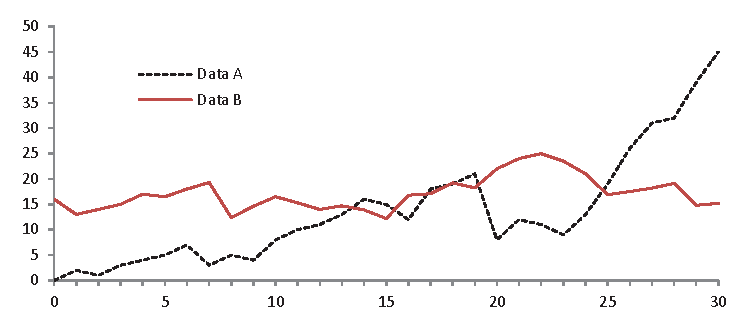
\includegraphics[width=\textwidth]{fig1.eps}
\caption{A figure caption is always placed below the illustration.
Please note that short captions are centered, while long ones are
justified by the macro package automatically.} \label{fig1}
\end{figure}

\begin{theorem}
This is a sample theorem. The run-in heading is set in bold, while
the following text appears in italics. Definitions, lemmas,
propositions, and corollaries are styled the same way.
\end{theorem}
%
% the environments 'definition', 'lemma', 'proposition', 'corollary',
% 'remark', and 'example' are defined in the LLNCS documentclass as well.
%
\begin{proof}
Proofs, examples, and remarks have the initial word in italics,
while the following text appears in normal font.
\end{proof}
For citations of references, we prefer the use of square brackets
and consecutive numbers. Citations using labels or the author/year
convention are also acceptable. The following bibliography provides
a sample reference list with entries for journal
articles~\cite{ref_article1}, an LNCS chapter~\cite{ref_lncs1}, a
book~\cite{ref_book1}, proceedings without editors~\cite{ref_proc1},
and a homepage~\cite{ref_url1}. Multiple citations are grouped
\cite{ref_article1,ref_lncs1,ref_book1},
\cite{ref_article1,ref_book1,ref_proc1,ref_url1}.

\begin{credits}
\subsubsection{\ackname} A bold run-in heading in small font size at the end of the paper is
used for general acknowledgments, for example: This study was funded
by X (grant number Y).

\subsubsection{\discintname}
It is now necessary to declare any competing interests or to specifically
state that the authors have no competing interests. Please place the
statement with a bold run-in heading in small font size beneath the
(optional) acknowledgments\footnote{If EquinOCS, our proceedings submission
system, is used, then the disclaimer can be provided directly in the system.},
for example: The authors have no competing interests to declare that are
relevant to the content of this article. Or: Author A has received research
grants from Company W. Author B has received a speaker honorarium from
Company X and owns stock in Company Y. Author C is a member of committee Z.
\end{credits}
%
% ---- Bibliography ----
%
% BibTeX users should specify bibliography style 'splncs04'.
% References will then be sorted and formatted in the correct style.
%
% \bibliographystyle{splncs04}
% \bibliography{mybibliography}
%
\begin{thebibliography}{8}
	\bibitem{kopp2020smt2020}
	Kopp, D., Hassoun, M., Kalir, A., Mönch, L.: SMT2020—a semiconductor manufacturing testbed. IEEE Transactions on Semiconductor Manufacturing 33(4):522–531 (2020)
	
	\bibitem{Hopp2011}
	Hopp, W. J., Spearman, M. L.: Factory physics. Waveland Press. (2011)
	
	\bibitem{Uzsoy1992}
	Uzsoy, R., Lee, C. Y., Martin-Vega, L. A.: A review of production planning and scheduling models in the semiconductor industry part I: system characteristics, performance evaluation and production planning. IIE transactions, 24(4), 47-60 (1992)
	
	\bibitem{schumann2022scheduling}
	Pinedo, M. L.: Scheduling: theory, algorithms, and systems. 6th edn. Springer (2022) 
	
	\bibitem{May2006}
	May, G. S., Spanos, C. J.: Fundamentals of semiconductor manufacturing and process control. John Wiley \& Sons. (2006)
	
	\bibitem{Mönch2011}
	Mönch, L., Fowler, J. W., Dauzère-Pérès, S., Mason, S. J., Rose, O.: A survey of problems, solution techniques, and future challenges in scheduling semiconductor manufacturing operations. Journal of scheduling, 14, 583-599. (2011)
	
	\bibitem{Ali2024}
	Ali, R., Qaiser, S., El-Kholany, M. M., Eftekhari, P., Gebser, M., Leitner, S., Friedrich, G. A Greedy Search Based Ant Colony Optimization Algorithm for Large-Scale Semiconductor Production. In Proceedings of the 14th International Conference on Simulation and Modeling Methodologies, Technologies and Applications (SIMULTECH 2024), pages 138-149. (2024)
	
	\bibitem{Dorigo2019}
	Dorigo, M., Stützle, T.: Ant colony optimization: overview and recent advances. In Handbook of Metaheuristics, pages 311–351. Springer (2019)
	
	\bibitem{Papadimitriou}
	Papadimitriou, C. H., Steiglitz, K.: Combinatorial Optimization: Algorithms and Complexity. Prentice-Hall. (1982)
	
	\bibitem{Perron2023}
	Perron, L., Didier, F., Gay, S.: The CP-SATLP
	solver (invited talk). In Proceedings of the 29th
	International Conference on Principles and Practice
	of Constraint Programming, pages 3:1–3:2. Leibniz
	International Proceedings in Informatics, (2023)
	
	\bibitem{Kovács2022}
	Kovács, B., Tassel, P., Ali, R., El-Kholany, M., Gebser, M., Seidel, G.: A customizable simulator for artificial intelligence research to schedule semiconductor fabs. In 2022 33rd Annual SEMI Advanced Semiconductor Manufacturing Conference (ASMC) (pp. 1-6). IEEE, (2022, May)
	
	\bibitem{waschneck2018deep}
	Waschneck, B., Reichstaller, A., Belzner, L., Altenmüller, T., Bauernhansl, T., Knapp, A., Kyek, A.: Deep reinforcement learning for semiconductor production scheduling. In 2018 29th annual SEMI advanced semiconductor manufacturing conference (ASMC) pp. 301-306. IEEE, (2018, April)
	
	\bibitem{leachman1996benchmarking}
	Leachman, R. C., Hodges, D. A.: Benchmarking semiconductor manufacturing. IEEE transactions on semiconductor manufacturing 9(2), 158-169 (1996)
	
	\bibitem{McKay2003}
	McKay, K. N., Wiers, V. C.: Planning, scheduling and dispatching tasks in production control. Cognition, Technology \& Work, 5, 82-93 (2003)
	
	\bibitem{chan2024situation}
	Chan, C. W.: Situation aware dispatching system for semiconductor manufacturing. (2024)


	\bibitem{ref_article1}
	Author, F.: Article title. Journal \textbf{2}(5), 99--110 (2016)
	
	\bibitem{ref_lncs1}
	Author, F., Author, S.: Title of a proceedings paper. In: Editor,
	F., Editor, S. (eds.) CONFERENCE 2016, LNCS, vol. 9999, pp. 1--13.
	Springer, Heidelberg (2016). \doi{10.10007/1234567890}
	
	\bibitem{ref_book1}
	Author, F., Author, S., Author, T.: Book title. 2nd edn. Publisher,
	Location (1999)
	
	\bibitem{ref_proc1}
	Author, A.-B.: Contribution title. In: 9th International Proceedings
	on Proceedings, pp. 1--2. Publisher, Location (2010)
	
	\bibitem{ref_url1}
	LNCS Homepage, \url{http://www.springer.com/lncs}, last accessed 2023/10/25
\end{thebibliography}
\end{document}
